\documentclass[public]{cfpbpresentation}
\usepackage{CDCShortcuts}

\beamerdefaultoverlayspecification{<+->}


%\newcommand{\bi}{\begin{itemize}}
%\newcommand{\ei}{\end{itemize}}

\renewcommand{\CRRA}{\gamma}
\renewcommand{\MPCP}{\chi}

\usepackage{natbib}
\begin{document}
\title{Two Awesome Papers Sort of About the MPC!}
\author{Chris Carroll}
\date{May 20, 2015}


\begin{frame}
  \titlepage
\end{frame}

\section{Why Do We Care?}

\begin{frame}\frametitle{Why Do We Care About the MPC?}

% Add figure on retail sales collapse 

\pause Nobody trying to make a forecast in 2009--2010 would ask: \pause

\centerline{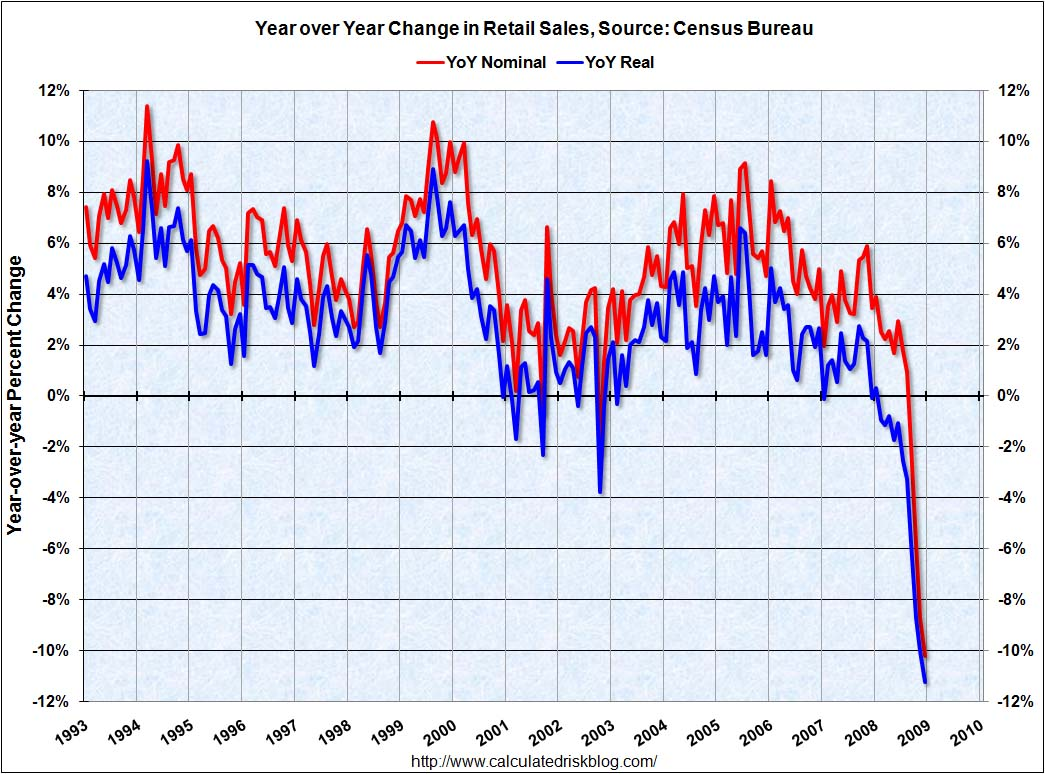
\includegraphics[width=3in]{./Figures/Retail-Sales-Collapse.jpg}}
\end{frame}

\begin{frame}\frametitle{Why Do We Care About the MPC?}

Nobody trying to make a forecast in 2009--2010 would ask: 

\begin{itemize}
%\item Big negative shocks to disposable income
\item Big `stimulus' tax cuts
\item Keynesian multipliers should be big
\bi
\item At least, in a (Keynesian) liquidity trap 
\ei
\item Crude Keynesianism: If $\cLev = \bar{\cLev} + (\yLev-\tau) \MPC$ 
\item $\Rightarrow$ multiplier on $\Delta \tau$ is $1/(1-\MPC) - 1$
\begin{itemize}
\item If $\MPC = 0.75$ then multiplier is $4-1=3$ \pause
\bi
\item Some micro estimates of $\MPC$ are this large
\ei
\item If $\MPC = 0.05$ then multiplier is only $\approx 0.05$
\bi
\item 2007-vintage DSGE models mostly implied $\MPC \in (0.00, 0.05)$
\ei
\end{itemize}
\end{itemize}

\end{frame}

\begin{frame}\frametitle{What, If Anything, Is `the MPC'}

\cite{friedmanATheory}:
\begin{eqnarray*}
    \yLev_{t} & = & \pLev_{t} + \Theta_{t}
\\  \cLev_{t} & = & \pLev_{t}
%\\  \pLev_{t+1} & = & \pLev_{t} + \Psi_{t+1}
\end{eqnarray*}

%\begin{eqnarray*}
%  \label{eq:CeqP}
%  \cLev_{t} & = & \pLev_{t}
%\end{eqnarray*}

\begin{itemize}
\item MPC out of transitory shocks is $\MPC = 0$
\item MPC out of permanent shocks is $\chi = 1$
\end{itemize}

\pause 
$\Rightarrow$ in a regression like
\begin{eqnarray*}
  \Delta \cLev_{t+1} & = & \alpha  \Delta \yLev_{t+1},
\end{eqnarray*}
we should find $0 < \alpha < 1$ depending on whether people {\it perceive}
$\Delta \yLev_{t+1}$ as transitory or permanent

\pause 

\vspace{0.1in}
Both papers are consistent with $0 < \hat{\alpha} < 1$.  Yay! (?)

\end{frame}

\begin{frame}\frametitle{What About Interest Income? }

If $\util(\cLev) = (1-\CRRA)^{-1}\cLev^{1-\CRRA}$, and $\rfree$ is believed to be constant forever, 
then \href{http://econ.jhu.edu/people/ccarroll/public/lecturenotes/consumption/PerfForesightCRRA}{perfect foresight infinite horizon model} says 
\begin{eqnarray*}
        \cLev & = & \underbrace{\left(\bLev_{\tNow}+ \pLevBF\left(\frac{1+\rfree}{\rfree}\right)\right)}_{\oLev}\overbrace{\left(\rfree-\CRRA^{-1}(\rfree-\timeRate)\right)}^{\MPC}
\\ & = & \oLev \MPC 
\end{eqnarray*}

\medskip\medskip
\pause
where $\oLev$ is `overall wealth' (human plus nonhuman), and $\oLev \MPC$ is the amount that is OK to spend (!)  

\end{frame}

\begin{frame}\frametitle{Unanticipated Permanent Change In $\rfree$}
\centerline{$\cLev_{\tNow} = \left(\rfree-\CRRA^{-1}(\rfree-\timeRate)\right)\left(\bLev_{\tNow}+ \pLevBF\left(\frac{1+\rfree}{\rfree}\right)\right)$}
\medskip\medskip\medskip


Three effects of an unanticipated permanent change in $\rfree$:
\begin{itemize}
\item Income Effect (assume $\CRRA^{-1} = 0$ and $\pLev=0$):
\begin{eqnarray*}
  \label{eq:inc}
    \Delta \cLev_{t+1} & = & \Delta \rfree_{t+1} \bLev_{t}
\end{eqnarray*}
\item Substitution Effect (assume $\pLev = 0$):
\begin{eqnarray*}
  \label{eq:sub}
    \Delta \cLev_{t+1} & = & \CRRA^{-1} \Delta \rfree_{t+1} \bLev_{t}
\end{eqnarray*}
\item Human Wealth Effect ($\pLev \neq 0$, $\rfree_{t}$ and $\rfree_{t+1}$ small)
\begin{eqnarray*}
  \label{eq:sub}
    \Delta \cLev_{t+1} & \approx & \left(1/\rfree_{t+1}-1/\rfree_{t}\right)\pLev \kappa_{t}
\\ & =  &  \left(\rfree_{t}/\rfree_{t+1}-1\right)(\kappa_{t}/\rfree_{t})\pLev 
\end{eqnarray*}
\end{itemize}
\end{frame}

\begin{frame}\frametitle{Sizes?  Depends on $\CRRA$ ...}

$\Delta \cLev_{t+1} = (1-\CRRA^{-1}) \Delta \rfree_{t+1}  \bLev_{t} + \left(\rfree_{t}/\rfree_{t+1}-1\right)(\kappa_{t}/\rfree_{t})\pLev \right)  $

\bi
\item Simple calibration: $\bLev_{t}=\pLev=1$, $\rfree_{t}=0.06$, $\rfree_{t+1}=\timeRate = 0.03$
\medskip\medskip
\begin{tabular}{|c|c|c|}
\hline 
 & \multicolumn{2}{c|}{Effect Size}
\\ $\CRRA$  &  Income-And-Substitution & Human Wealth
\\ \hline $\infty$ & 0.03 & 1
\\  $1$ & 0 & 0.5
\\ \hline 
\end{tabular}
\ei

\bi
\item Hi
\ei


\end{frame}

\beamerdefaultoverlayspecification{<*>}

\begin{frame}[allowframebreaks]

\bibliographystyle{plainnat}
\bibliography{economics}
\end{frame}

%\input bibMake

\end{document}

\section{Optimality}


\begin{frame}
  \frametitle{\insertsection}
  \begin{itemize}[<+->]
  \item  Neoclassical, ``useful'' behavioral ...
\begin{itemize}
\item ... require calculation of the optimal choice
\item ... both imply that moving toward optimal is good!
\end{itemize}
  \item Unfortunately, solving optimal choice models is v. hard
    \begin{itemize}[<+->]
    \item Even for PhD economists who are experts in CF
      \begin{itemize}[<+->]
      \item Notorious examples (not in slides)
      \end{itemize}
    \end{itemize}

  \item  Current situation: like econometrics in 1950s, 60s
    \begin{itemize}[<+->]
    \item Lots of abstract ``in principle'' knowledge, theorems
    \item But actual applications are hand-crafted
    \end{itemize}

  \item Solving these models should be like doing a regression
    \begin{itemize}[<+->]
    \item Shouldn't require years of human capital investment
\begin{itemize}
\item in things that are {\it not} economics
\end{itemize}
%    \item Transparent, replicable, extensible, documented
    \end{itemize}
    \item CFPB: 21st century government agency!
  \end{itemize}
\end{frame}


\section{Who Has Figured This Out?}

\begin{frame}
  \frametitle{\insertsection}
  \begin{itemize}[<+->]
    \item Open-source software development world
    \item  Open source successes:
      \begin{itemize}[<+->]
      \item Linux
      \item LaTeX
      \item Successful programming languages
%      \item Firefox
      \end{itemize}
\end{itemize}

\end{frame}  

\section{Lessons from the Professionals}

\begin{frame}
  \frametitle{\insertsection}
  \begin{itemize}[<+->]
  \item Open-source infrastructure:
  \begin{itemize}[<+->]
    \item Repositories: store, share, checkpoint code automatically
    \item Transparency, reproducibility via documentation
    \item Share ideas, code, math together: notebooks and gists
      \begin{itemize}[<+->]
        \item \href{https://github.com/ipython/ipython/wiki/A-gallery-of-interesting-IPython-Notebooks\#reproducible-academic-publications}{Reproducible academic research}
%        \item Incentivize collaboration: Hackathons, Google Summer of          Code, bounties 
        \end{itemize}
      \end{itemize}
    \end{itemize}
\end{frame}

\section{Version 1.0}


\begin{frame}
  \frametitle{\insertsection}
Heterogeneous Agents Computing toolKit (HACK) will be rolled out at a conference later this year:
  \begin{itemize}[<+->]
  \item Well-documented, well tested tools
  \item Examples using these tools to solve canonical models
  \begin{itemize}[<+->]
    \item \href{http://nbviewer.ipython.org/gist/npalmer/fae19b5673d9226dcbcd}{Portfolio Choice}
    \item Life cycle model with stochastic income, liq constrs
    \item Indirect inference of RRA, time preference
    \item Krusell-Smith
    \item Campbell-Cocco
    \item Carroll, Slacalek, Tokuoka, White
    \end{itemize}
\end{itemize}

\end{frame}

\section{Needs Critical Mass}

\begin{frame}
  \frametitle{\insertsection}
  \begin{itemize}[<+->]
    \item Encouraging collaboration is the next crucial step
      \begin{itemize}[<+->]
        \item Problem sets
        \item Graduate student prizes
        \item Performance plans
      \end{itemize}
    \end{itemize}
  \begin{itemize}[<+->]
        \item Your suggestions?
    \end{itemize}

\end{frame}

\begin{frame}
\frametitle{References}


\bibliographystyle{plainnat}
\bibliography{sample}

\end{frame}

\end{document}
